\section{Diagramme de Use-Case}


\begin{figure}[!ht]
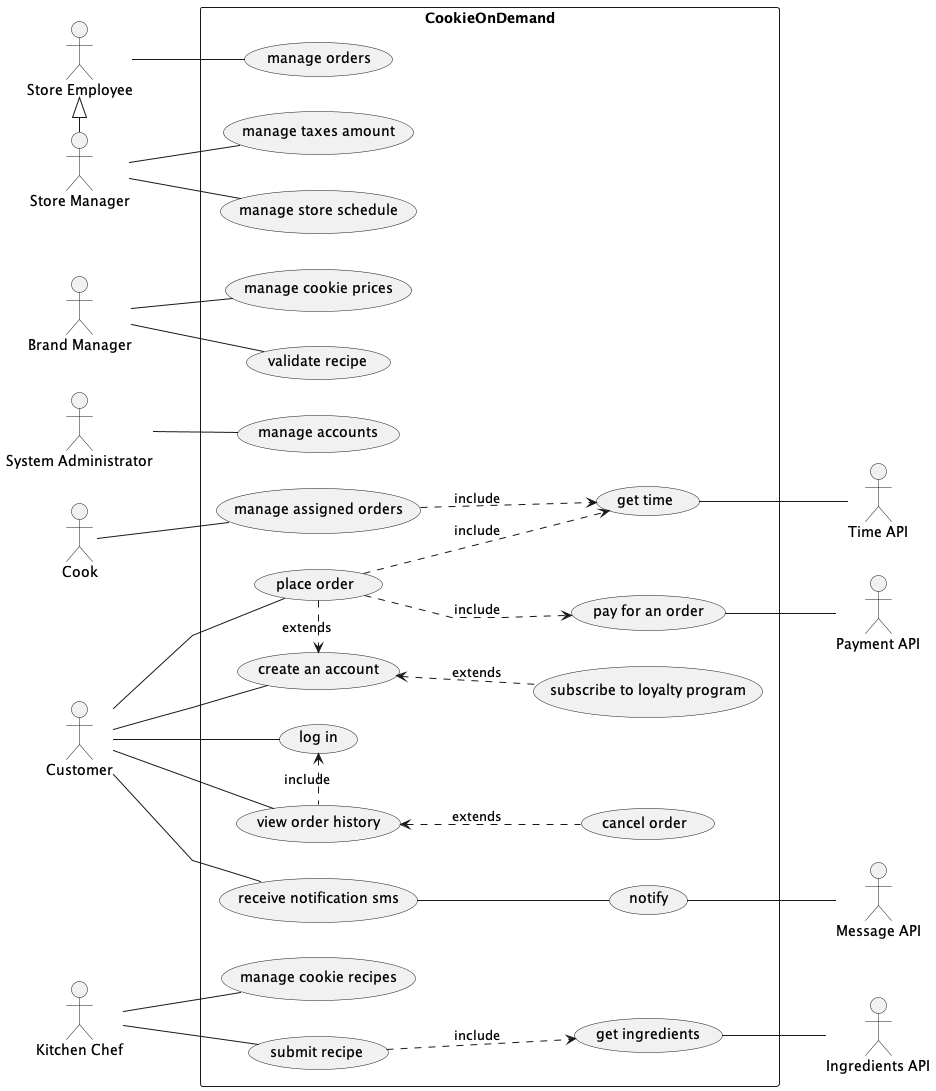
\includegraphics[width=0.7\textwidth]{use-cases}
\centering
\caption{Diagramme de Use-Case couvrant le périmètre final}
\label{uml:use-cases}
\end{figure}

\paragraph{Ce diagramme de Use case} part du principe que tous les utilisateurs sont connectés et que leurs comptes 
bénéficient des droits d’accès pour effectuer leurs tâches respectives.
